\chapter{Main Body}
\label{cha:Main Body}

\section{Trigger R\&D}
\label{sec:Trigger}
To trigger the counter of the WSB, there are a few possible solutions. The remote has to be wearable, and it has to be triggered during the game. This is hard to implement, because a usual button is too tiny to press during a game, and it can be frustrating to always aim for the trigger button. Therefore, I decided to use an accelerometer and count the points by simply tapping on the thigh. My idea is to mount the WSB remote on the inside of the thigh or as a knee pad replacement for example in volleyball. Then the vibrations/accelerations travel through the user's body and get measured by the WSB remote. But this can be rather hard, because during sports the body is always accelerating, and it could be hard to distinguish from a usual movement or a "thigh tip". If the accelerometer idea doesn't work out, I would use flexible membrane buttons to control the WSB. 

\subsection{Accelerometer R\&D}
\label{ssec:Accelerometer}
At my current lab at ETH I found an accelerometer to test out, if I can use it as a trigger.
\subsubsection{control LSM303C accelerometer}
Attention: Mind that the CS\_XL and CS\_MAG have to be pulled up to enable I\textsuperscript{2}C mode. and use external I\textsuperscript{2}C pullups, because on MKI163V1 devBoard are no pullup R's.

slave address: 0b00111010 = 0x3A \cite{DS_LSM303C}

\begin{figure}[H]
	\centering
	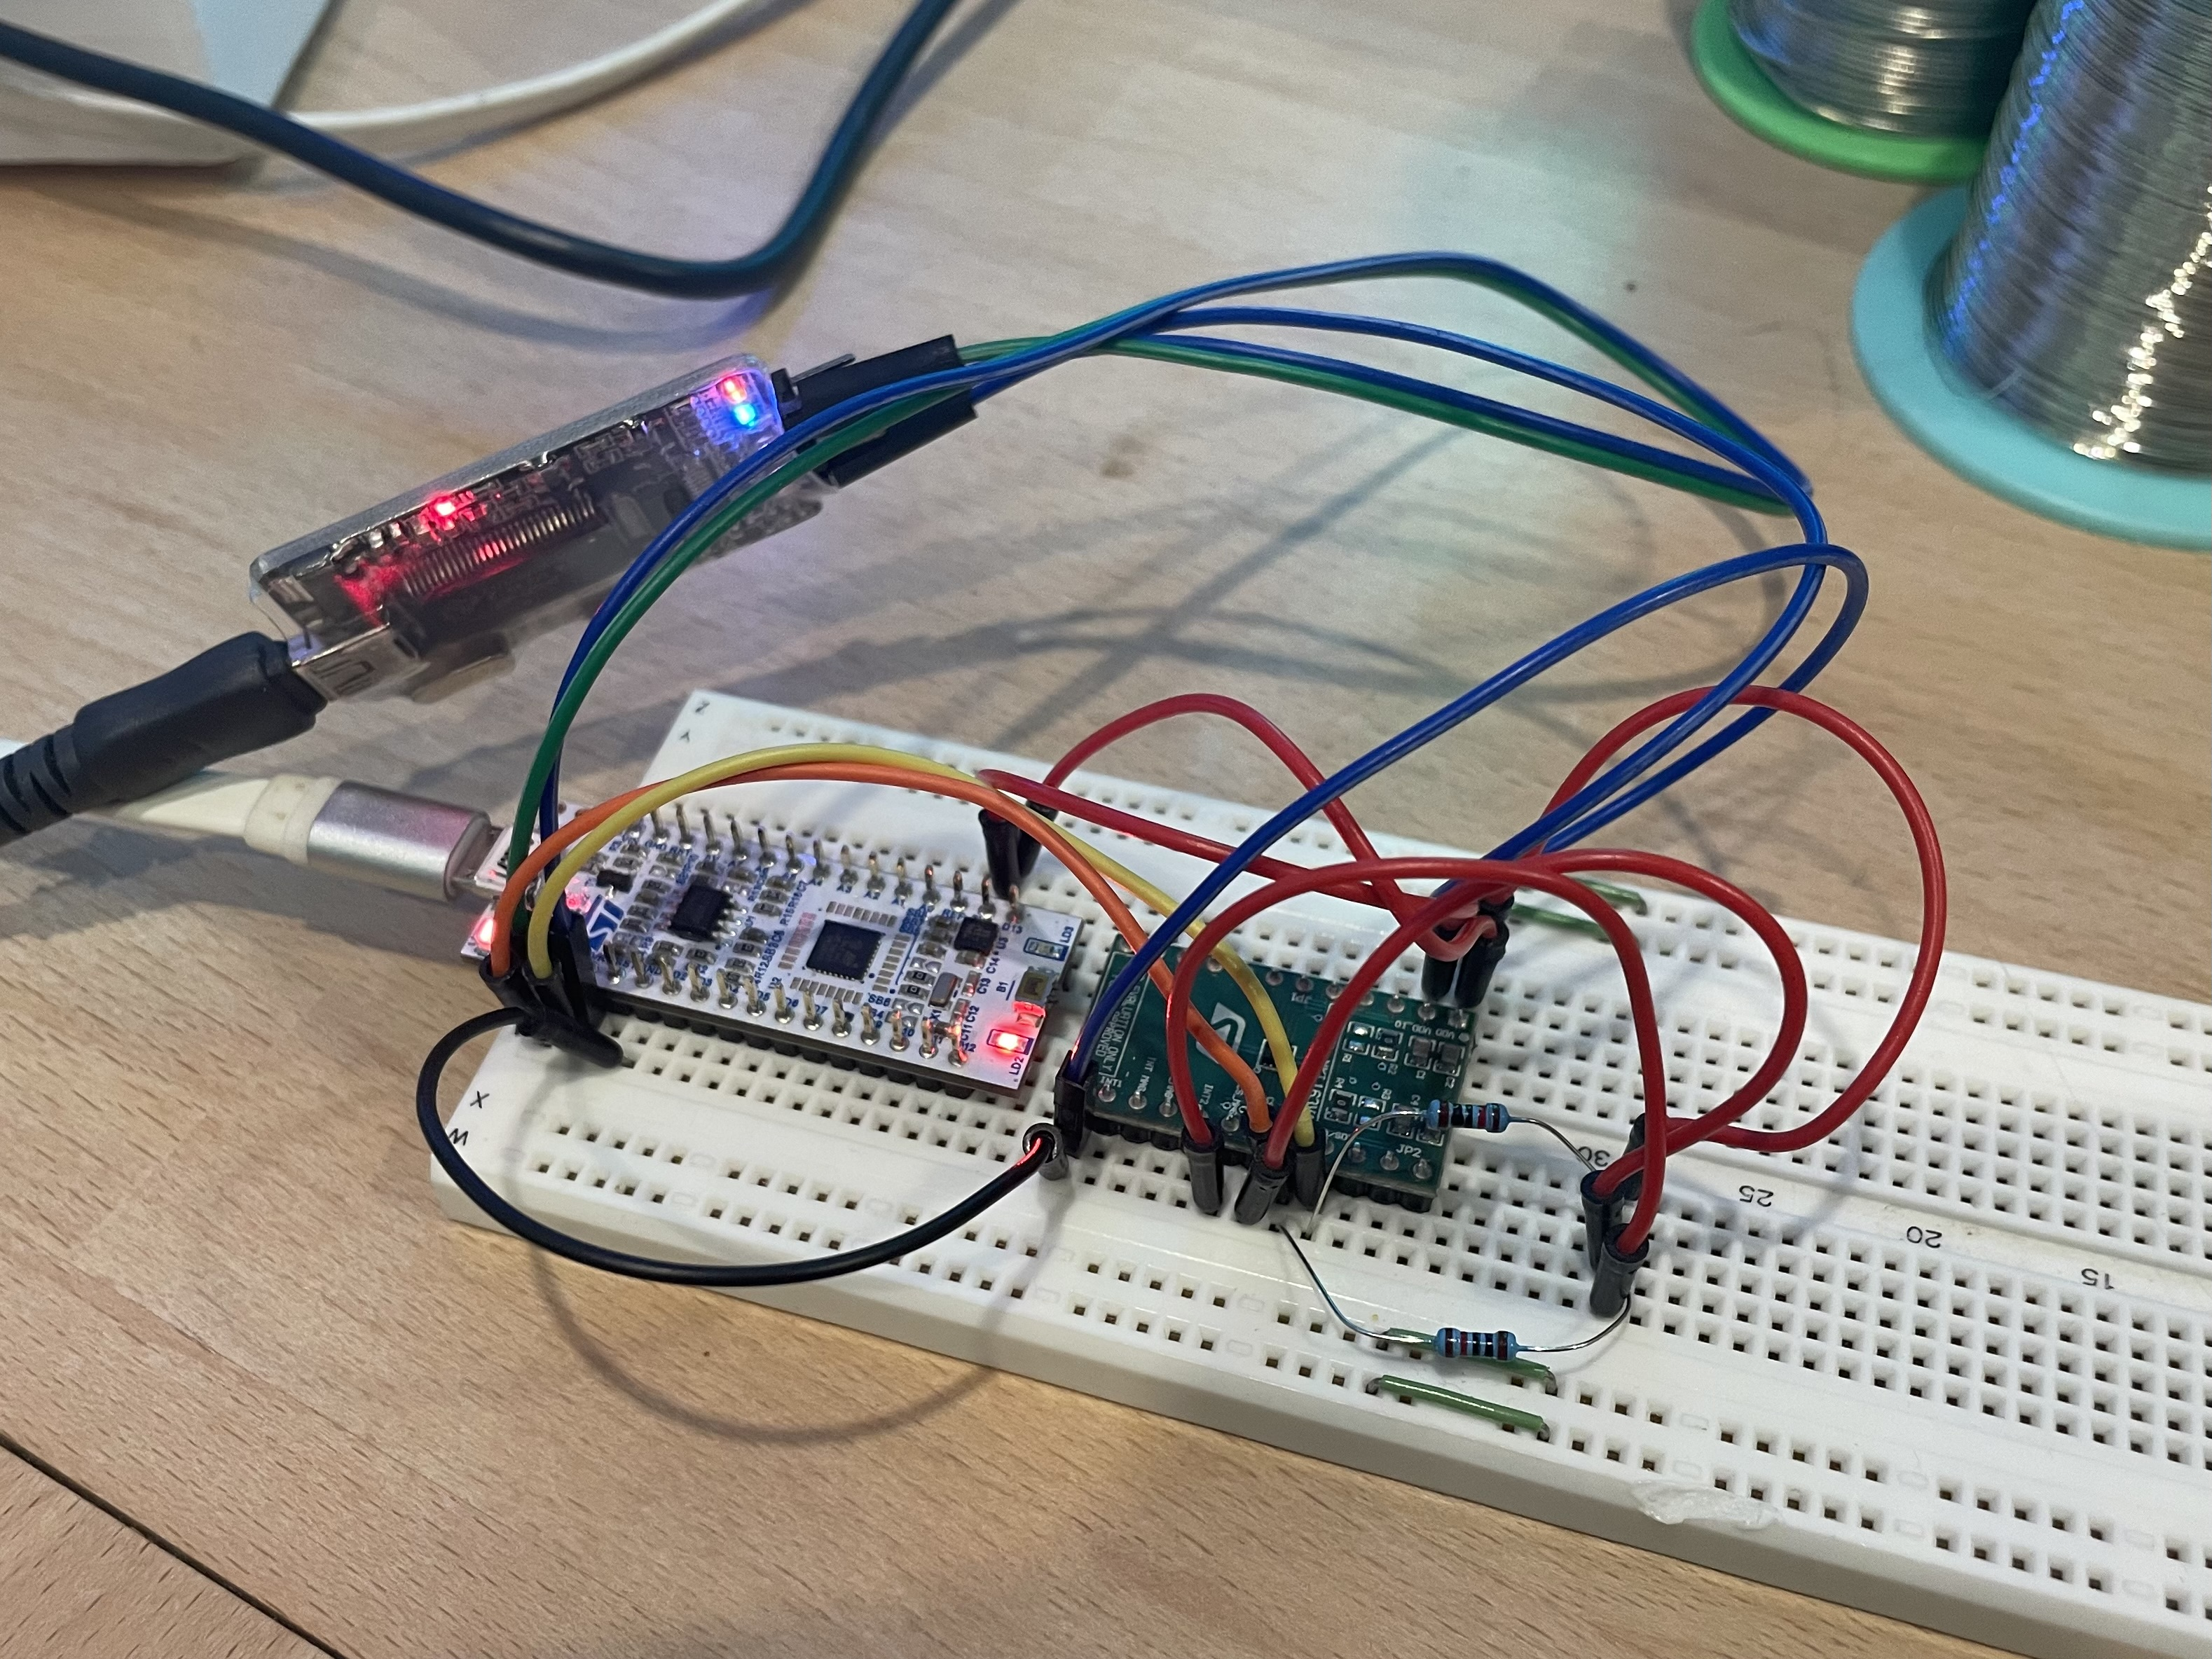
\includegraphics[width=10cm]{Resources/accTestLab.jpeg}
	\caption{Accelerometer test: setup}
	\label{fig:accTestLab}
\end{figure}

\subsubsection{First test the "WHO AM I" register}
Communication test: reg 0x0F should read as 0x41

\subsubsection{Read acceleration}
CTRL\_REG1\_A (0x20): 0x3F (Enable XYZ, 100Hz, block data overwriting)

CTRL\_REG2\_A (0x21): 0x00 (disable LPF)

CTRL\_REG3\_A (0x22): 0x00 (disable interrupts)

CTRL\_REG4\_A (0x23): 0x34 (enable I\textsuperscript{2}C, enable auto address increments, FS $\pm$8g)

CTRL\_REG5\_A (0x24): 0x00

CTRL\_REG6\_A (0x25): 0x00

CTRL\_REG7\_A (0x26): 0x00
\\

STATUS\_REG\_A (0x27):
Bit 3 set if xyz data is available / Bit 8 set if xyz data overrun.

OUT\_X\_L (0x28)(2bytes)   (0.061mg/LSB) @ FS=8g

OUT\_Y\_L (0x2A)(2bytes)   (0.061mg/LSB) @ FS=8g

OUT\_Z\_L (0x2C)(2bytes)   (0.061mg/LSB) @ FS=8g

\begin{figure}[H]
	\centering
	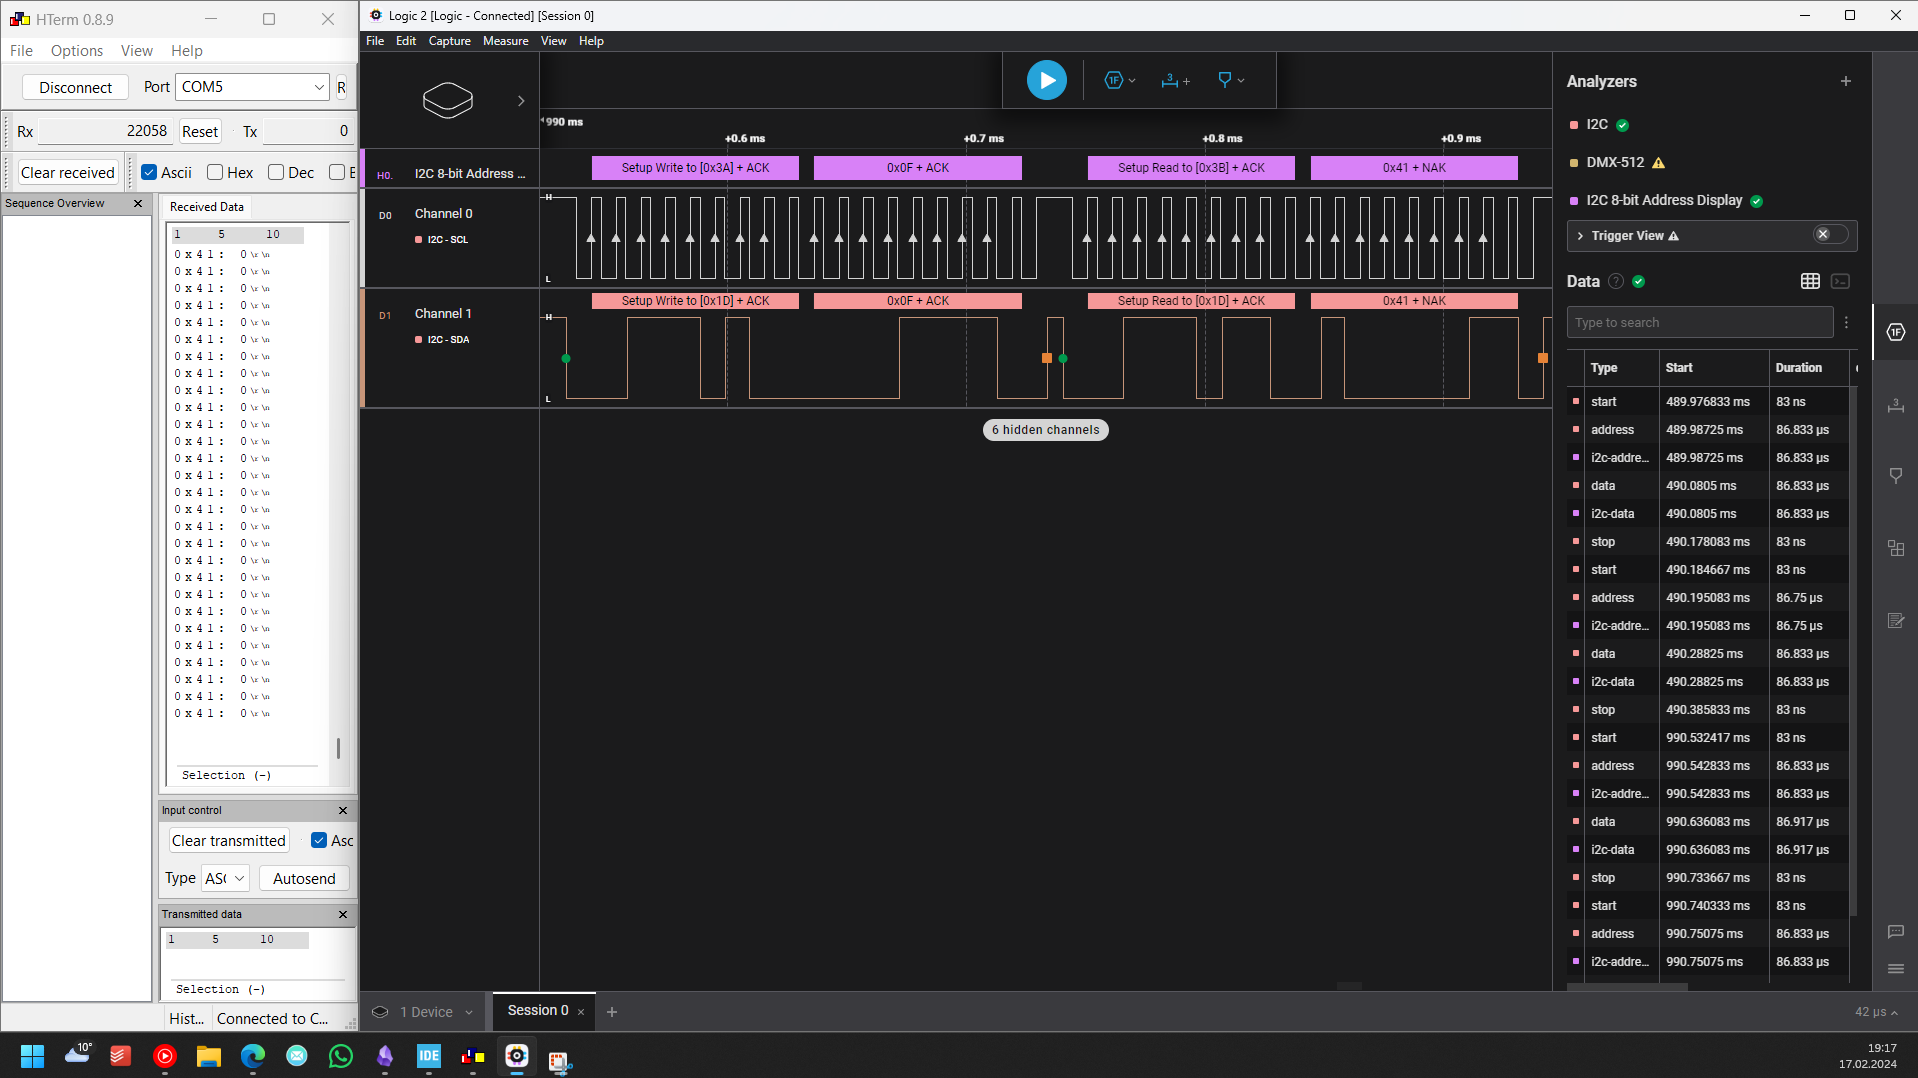
\includegraphics[width=17cm]{Resources/accTestLA.png}
	\caption{Accelerometer test: logic analyzer}
	\label{fig:accTestLA}
\end{figure}
\newpage

\subsubsection{Test Results}
After looking at the measurement results, I decided that it would be best to populate an accelerometer and the membrane buttons on the PCB, that I have an alternative if the accelerometer doesn't work out. Because it's hard to analyze if the accelerometer as trigger will work out during a game and I can't attach the current breadboard to my thigh to test the accelerometer out. But for the final design I'll probably choose the "STM LIS2HH12" accelerometer.

\begin{figure}[H]
	\centering
	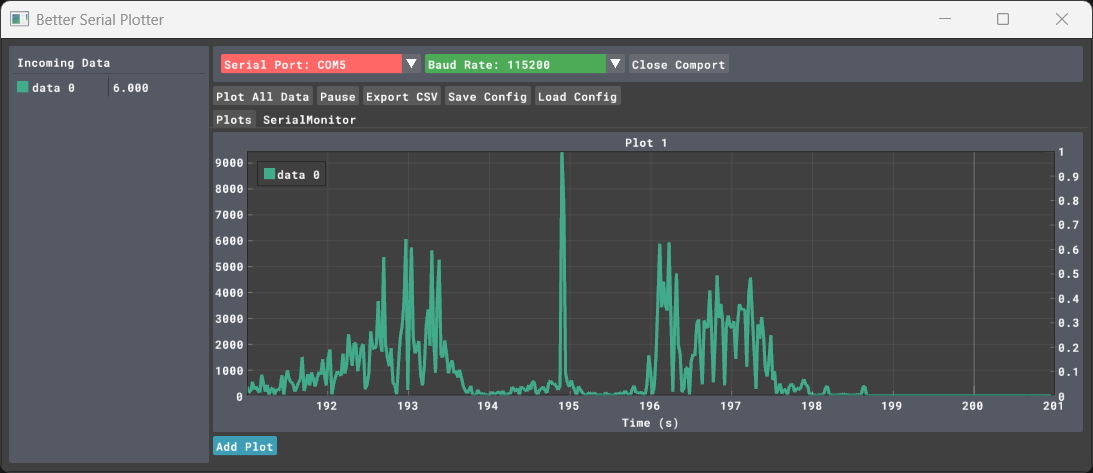
\includegraphics[width=17cm]{Resources/accTestMeas.png}
	\caption{Accelerometer test: results}
	\label{fig:accTestMeas}
\end{figure}

I hope that I can differentiate normal sports movement from "thigh taps" by looking at the momental acceleration. In Fig: \ref{fig:accTestMeas}, the middle pulse was a "thigh tap" and the first and last ones are movement from the body, which take a lot longer but don't peak out as high. The shown data is actually the variable "accDelta" from the "6\_Software/dev/LSM303C\_Test/Core/Src/ main.c" file.

\section{Battery Charging R\&D}
\label{sec:Battery Charging}
I'm sure, that I'll have to somehow power the WSB Remote as well as the WSB. Because they both have to be portable, I'm planning to use a rechargeable battery. For example Lithium Ion battery. And to use this battery I'll have to implement some protection circuits, as well as charging circuits. Important protection features are:
\begin{itemize}
    \item UVP - Under Voltage Protection (So the battery doesn't get broken)
    \item OVP - Over Voltage Protection (So the battery doesn't get broken)
    \item OTP - Over Temperature Protection (So the battery doesn't overheat or starts burning)
    \item OCP - Over Current Protection (So the circuits don't break)
\end{itemize}

So I started searching for LiIon charging ICs and I had looks at TIs ICs, like the "BQ25180YBGR" or "BQ25155YFPR". But the TI charging ICs are rather complicated and would take me too long to implement. Additionally after buying some samples of these ICs I recognized, that they are CSPs and really tiny, which makes them really hard to solder or make modifications on the PCB. So I got to my favourite semiconductor manufacturer STM and found the perfect IC, the STNS01. I also recognized, that STMs product portfolio is a lot smaller than TIs, which was quite overwhelming. STM only had about 5 ICs to choose from.

\subsection{STNS01 R\&D}
\label{ssec:STNS01}

\section{HW Concept}
\label{sec:HW Concept}

\begin{figure}[H]
	\centering
	\includegraphics[width=17cm]{../}
	\caption{Accelerometer test: logic analyzer}
	\label{fig:accTestLA}
\end{figure}